% ============================================================
% sq14-layout.tex (2026-11-18): review diagram, not a paper figure.
% (a) the paper's one-ancilla layout, drawn as panel (b) of
%     paper-rework/a1-layout-figure/ancilla-layouts-B.tex;
% (b) layout SQ14 from ../README section "One ancilla per check on a square
%     lattice" (rounds.py SQ14): 3x3 square patch
%         a3  a4  q1
%         q3  q0  q4
%         q2  a2  a1
%     a1: q4; a2: q0, q2; a3: q3; a4: q0, q1; transfers a1-a2 and a3-a4;
%     in-round data windows CNOT_INV q1->q4 and CNOT q3->q2 (control -> target).
% Palette and node styles: exactly those of ancilla-layouts-B.tex.
% ============================================================
\documentclass[tikz,border=1pt]{standalone}
\usepackage{amsmath,amssymb}
\usetikzlibrary{calc,arrows.meta,decorations.markings}

\definecolor{Zcol}{HTML}{FF1744}
\definecolor{Xcol}{HTML}{00B7FF}
\definecolor{SwapCol}{HTML}{8E44AD}
\colorlet{Xtint}{Xcol!26}
\colorlet{Ztint}{Zcol!17}
\colorlet{XRim}{Xcol}
\colorlet{ZRim}{Zcol}
\colorlet{XText}{Xcol!80!black}
\colorlet{ZText}{Zcol!85!black}
\colorlet{GateCol}{SwapCol}
\colorlet{WinCol}{black!62}

\def\u{1.40}
\def\rq{0.17}
\def\ss{0.40}
\def\lab{0.37}

\tikzset{
  every node/.style={font=\footnotesize},
  data/.style={circle,inner sep=0pt,minimum size=2*\rq cm,line width=0.7pt,
               draw=black,fill=white,font=\scriptsize},
  site/.style={rectangle,rounded corners=1.2pt,inner sep=0pt,minimum size=\ss cm,
               line width=0.7pt,font=\footnotesize},
  xsite/.style={site,draw=XRim,fill=Xtint},
  zsite/.style={site,draw=ZRim,fill=Ztint},
  used/.style={line width=0.9pt,draw=black},
  gate/.style={line width=1.2pt,draw=GateCol,line cap=round},
  % in-round data CNOT, applied and undone inside the round; arrow = control -> target
  midarrow/.style={postaction={decorate},decoration={markings,
      mark=at position 0.56 with {\arrow{Stealth[length=4.2pt,width=4.6pt]}}}},
  window/.style={line width=1.2pt,draw=WinCol,line cap=round,midarrow},
  % ancilla-ancilla coupler: partial sums of one check type move between the two ancillas
  ztransfer/.style={line width=1.0pt,draw=ZRim,dash pattern=on 3pt off 1.6pt},
  xtransfer/.style={line width=1.0pt,draw=XRim,dash pattern=on 3pt off 1.6pt},
  readout/.style={font=\footnotesize,inner sep=0pt},
  title/.style={font=\footnotesize,anchor=base west,inner sep=0pt},
  stats/.style={font=\scriptsize,anchor=north,inner sep=0pt,text=black!75},
}

\newcommand{\DataNodes}{\foreach \i in {0,...,4} \node[data] at (q\i) {\i};}
\newcommand{\Readout}[3]{\node[readout,anchor=#2+180] at ($(#1)+(#2:\lab)$) {#3};}
\newcommand{\Panel}[3]{\node[title] at (#1) {{\small\bfseries(#2)}\hspace{0.45em}#3};}
\newcommand{\SH}{\bar S,\,\bar H}
\newcommand{\KeyLine}[1]{\tikz[baseline=-0.5ex]\draw[#1] (0,0) -- (0.50,0);}

\begin{document}
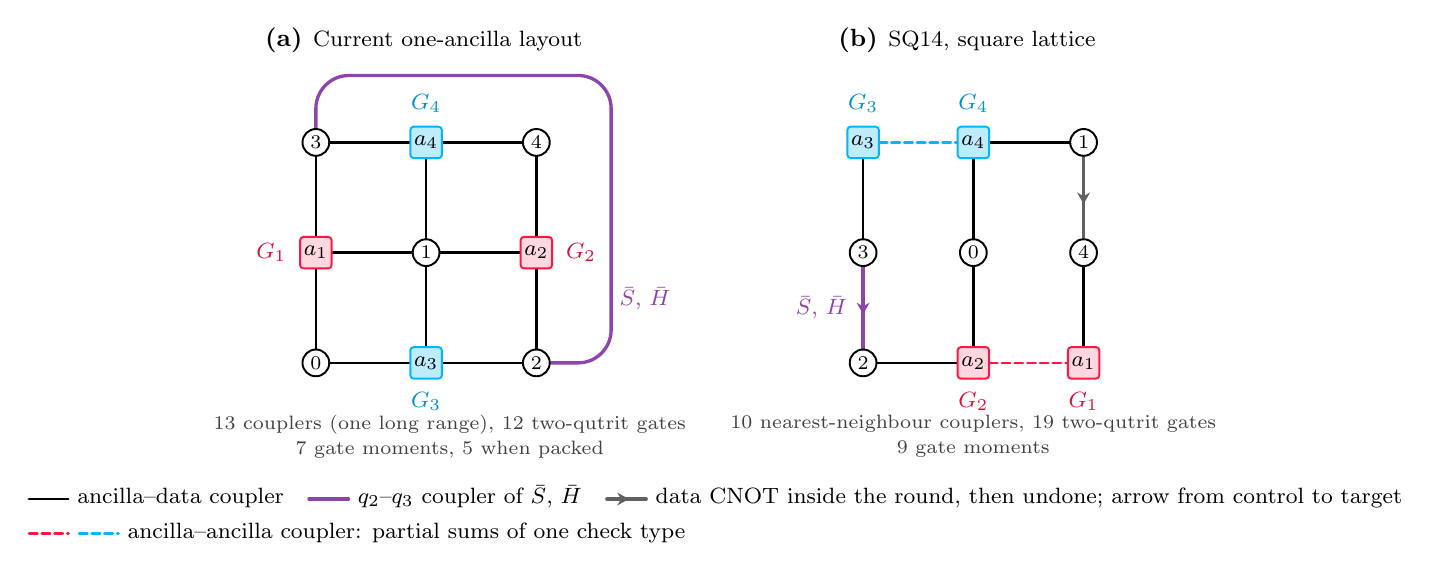
\begin{tikzpicture}[line cap=round,line join=round]
\def\yT{2.62} \def\yS{-2.05} \def\yK{-2.95}
\coordinate (A) at (0,0);
\coordinate (B) at (6.95,0);

% ==================== (a) current one-ancilla layout ====================
\begin{scope}[shift={(A)}]
  \coordinate (q3) at (-\u, \u); \coordinate (q4) at ( \u, \u);
  \coordinate (q1) at (0,0);
  \coordinate (q0) at (-\u,-\u); \coordinate (q2) at ( \u,-\u);
  \coordinate (a4) at (0, \u); \coordinate (a1) at (-\u,0);
  \coordinate (a2) at (\u,0);  \coordinate (a3) at (0,-\u);
  \def\h{0.95}
  \draw[gate,rounded corners=0.42cm,shorten <=\rq cm+0.5pt,shorten >=\rq cm+0.5pt]
    (q3) -- (-\u,\u+0.85) -- (\u+\h,\u+0.85) -- (\u+\h,-\u) -- (q2);
  \node[readout,text=GateCol,anchor=west] at (\u+\h+0.10,-0.42*\u) {$\SH$};
  \foreach \a/\b in {a4/q3,a4/q1,a4/q4,a1/q3,a1/q1,a1/q0,a2/q4,a2/q1,a2/q2,a3/q0,a3/q1,a3/q2}
    \draw[used] (\a) -- (\b);
  \node[xsite] at (a4) {$a_4$}; \node[zsite] at (a1) {$a_1$};
  \node[zsite] at (a2) {$a_2$}; \node[xsite] at (a3) {$a_3$};
  \DataNodes
  \Readout{a4}{90}{\textcolor{XText}{$G_4$}}
  \Readout{a1}{180}{\textcolor{ZText}{$G_1$}}
  \Readout{a2}{0}{\textcolor{ZText}{$G_2$}}
  \Readout{a3}{270}{\textcolor{XText}{$G_3$}}
  \node[stats] at (0.30,\yS) {13 couplers (one long range), 12 two-qutrit gates};
  \node[stats] at (0.30,\yS-0.34) {7 gate moments, 5 when packed};
\end{scope}
\Panel{$(A)+(-2.05,\yT)$}{a}{Current one-ancilla layout}

% ==================== (b) SQ14 ====================
\begin{scope}[shift={(B)}]
  \coordinate (a3) at (-\u, \u); \coordinate (a4) at (0, \u); \coordinate (q1) at (\u, \u);
  \coordinate (q3) at (-\u, 0);  \coordinate (q0) at (0, 0);  \coordinate (q4) at (\u, 0);
  \coordinate (q2) at (-\u,-\u); \coordinate (a2) at (0,-\u); \coordinate (a1) at (\u,-\u);
  % ancilla-data couplers of the reads
  \foreach \a/\b in {a3/q3,a4/q1,a4/q0,a2/q0,a2/q2,a1/q4} \draw[used] (\a) -- (\b);
  % transfers between the two ancillas of one type
  \draw[xtransfer,shorten <=0.5*\ss cm,shorten >=0.5*\ss cm] (a3) -- (a4);
  \draw[ztransfer,shorten <=0.5*\ss cm,shorten >=0.5*\ss cm] (a2) -- (a1);
  % in-round data windows: CNOT_INV q1 -> q4 and CNOT q3 -> q2 (q2-q3 also carries S, H)
  \draw[window,shorten <=\rq cm+0.5pt,shorten >=\rq cm+0.5pt] (q1) -- (q4);
  \draw[gate,midarrow,shorten <=\rq cm+0.5pt,shorten >=\rq cm+0.5pt] (q3) -- (q2);
  \node[readout,text=GateCol,anchor=east] at ($(q3)!0.5!(q2)+(-0.20,0)$) {$\SH$};
  \node[xsite] at (a3) {$a_3$}; \node[xsite] at (a4) {$a_4$};
  \node[zsite] at (a2) {$a_2$}; \node[zsite] at (a1) {$a_1$};
  \DataNodes
  \Readout{a3}{90}{\textcolor{XText}{$G_3$}}
  \Readout{a4}{90}{\textcolor{XText}{$G_4$}}
  \Readout{a2}{270}{\textcolor{ZText}{$G_2$}}
  \Readout{a1}{270}{\textcolor{ZText}{$G_1$}}
  \node[stats] at (0,\yS) {10 nearest-neighbour couplers, 19 two-qutrit gates};
  \node[stats] at (0,\yS-0.34) {9 gate moments};
\end{scope}
\Panel{$(B)+(-1.72,\yT)$}{b}{SQ14, square lattice}

% ==================== key ====================
\path (current bounding box.west) coordinate (bbW) (current bounding box.east) coordinate (bbE);
\coordinate (bbM) at ($(bbW)!0.5!(bbE)$); \coordinate (keyY) at (0,\yK);
\node[anchor=north,inner sep=0pt,font=\footnotesize,align=left] at (bbM |- keyY) {%
  \KeyLine{used}\ ancilla--data coupler\hspace{1.0em}%
  \KeyLine{gate}\ $q_2$--$q_3$ coupler of $\SH$\hspace{1.0em}%
  \KeyLine{window}\ data CNOT inside the round, then undone; arrow from control to target\\[3pt]%
  \KeyLine{ztransfer}\ \KeyLine{xtransfer}\ ancilla--ancilla coupler: partial sums of one check type};
\end{tikzpicture}
\end{document}
